\documentclass{standalone}
\usepackage{tikz}
\usetikzlibrary{patterns, positioning}


\begin{document}
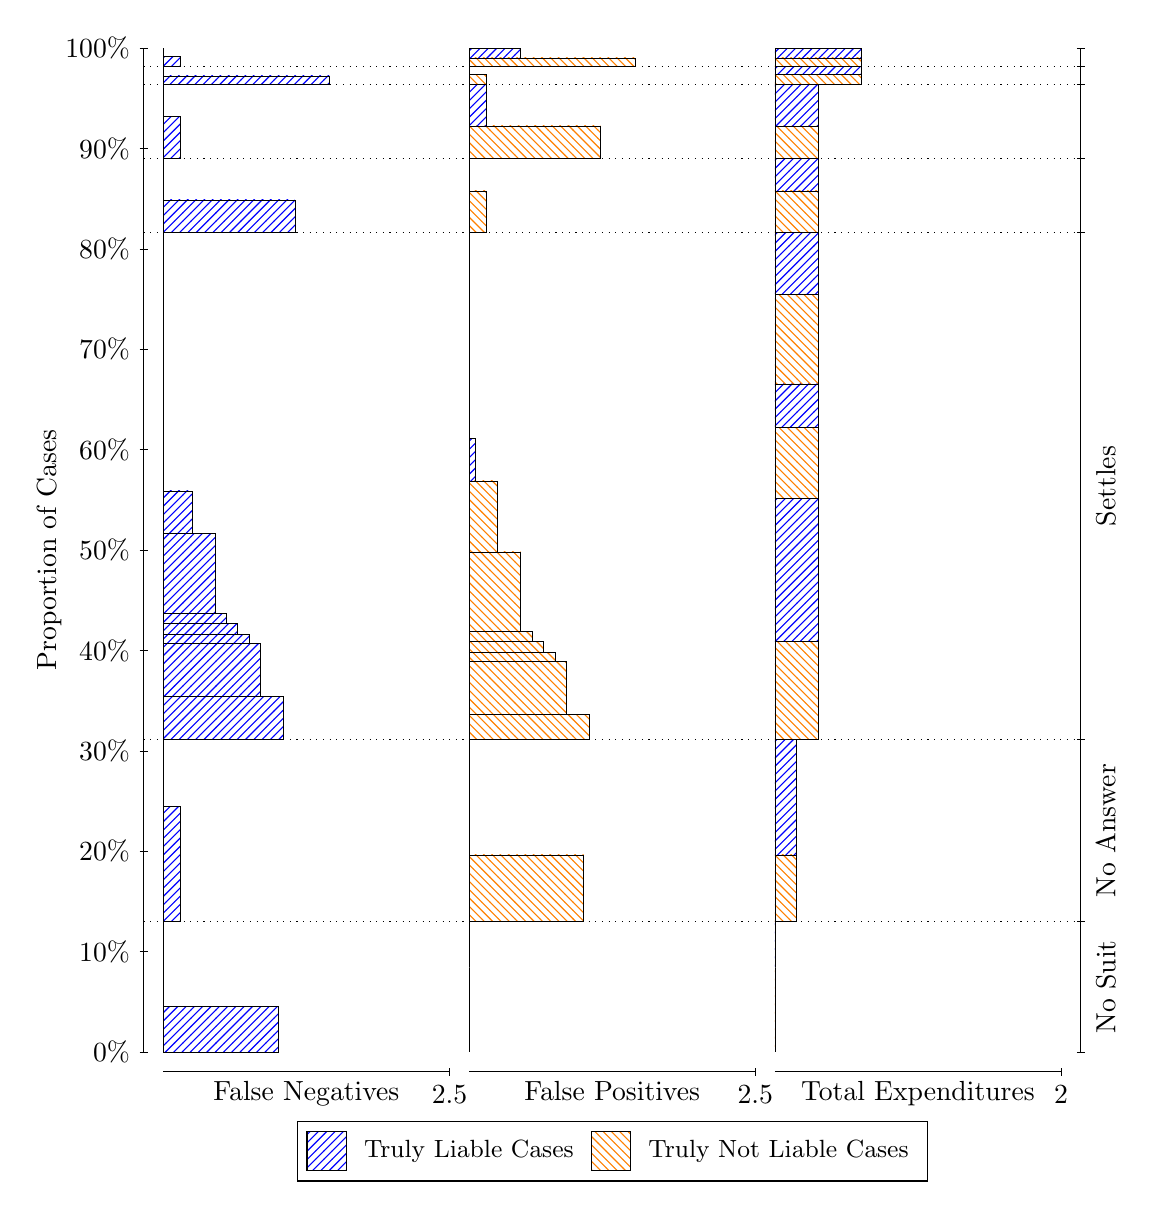
\begin{tikzpicture}
\draw[black, very thin] (1.5,1.75) -- (1.5,14.5);
\node[rotate=90, text=black, anchor=center] at (0.3, 8.125) {Proportion of Cases};
\draw[black, very thin] (1.45,1.75) -- (1.55,1.75);
\node[text=black, anchor=east] at (1.45, 1.75) {0\%};
\draw[black, very thin] (1.45,3.025) -- (1.55,3.025);
\node[text=black, anchor=east] at (1.45, 3.025) {10\%};
\draw[black, very thin] (1.45,4.3) -- (1.55,4.3);
\node[text=black, anchor=east] at (1.45, 4.3) {20\%};
\draw[black, very thin] (1.45,5.575) -- (1.55,5.575);
\node[text=black, anchor=east] at (1.45, 5.575) {30\%};
\draw[black, very thin] (1.45,6.85) -- (1.55,6.85);
\node[text=black, anchor=east] at (1.45, 6.85) {40\%};
\draw[black, very thin] (1.45,8.125) -- (1.55,8.125);
\node[text=black, anchor=east] at (1.45, 8.125) {50\%};
\draw[black, very thin] (1.45,9.4) -- (1.55,9.4);
\node[text=black, anchor=east] at (1.45, 9.4) {60\%};
\draw[black, very thin] (1.45,10.675) -- (1.55,10.675);
\node[text=black, anchor=east] at (1.45, 10.675) {70\%};
\draw[black, very thin] (1.45,11.95) -- (1.55,11.95);
\node[text=black, anchor=east] at (1.45, 11.95) {80\%};
\draw[black, very thin] (1.45,13.225) -- (1.55,13.225);
\node[text=black, anchor=east] at (1.45, 13.225) {90\%};
\draw[black, very thin] (1.45,14.5) -- (1.55,14.5);
\node[text=black, anchor=east] at (1.45, 14.5) {100\%};

\draw[black, very thin] (13.4,1.75) -- (13.4,14.5);
\draw[black, very thin] (13.35,1.75) -- (13.45,1.75);
\node[anchor=west] at (13.35, 1.75) {};
\draw[black, very thin] (13.35,3.4067) -- (13.45,3.4067);
\node[anchor=west] at (13.35, 3.4067) {};
\draw[black, very thin] (13.35,5.7187) -- (13.45,5.7187);
\node[anchor=west] at (13.35, 5.7187) {};
\draw[black, very thin] (13.35,12.158) -- (13.45,12.158);
\node[anchor=west] at (13.35, 12.158) {};
\draw[black, very thin] (13.35,13.1) -- (13.45,13.1);
\node[anchor=west] at (13.35, 13.1) {};
\draw[black, very thin] (13.35,14.041) -- (13.45,14.041);
\node[anchor=west] at (13.35, 14.041) {};
\draw[black, very thin] (13.35,14.27) -- (13.45,14.27);
\node[anchor=west] at (13.35, 14.27) {};
\draw[black, very thin] (13.35,14.5) -- (13.45,14.5);
\node[anchor=west] at (13.35, 14.5) {};

\draw[black, very thin, pattern color=blue, pattern=north east lines] (1.75,1.75) rectangle (3.2033,2.3339);
\draw[black, very thin, pattern color=orange, pattern=north west lines] (1.75,2.3339) rectangle (1.75,3.4067);
\draw[black, very thin, pattern color=blue, pattern=north east lines] (1.75,3.4067) rectangle (1.968,4.8712);
\draw[black, very thin, pattern color=orange, pattern=north west lines] (1.75,4.8712) rectangle (1.75,5.7187);
\draw[black, very thin, pattern color=blue, pattern=north east lines] (1.75,5.7187) rectangle (3.276,6.2708);
\draw[black, very thin, pattern color=blue, pattern=north east lines] (1.75,6.2708) rectangle (2.9853,6.937);
\draw[black, very thin, pattern color=blue, pattern=north east lines] (1.75,6.937) rectangle (2.84,7.0548);
\draw[black, very thin, pattern color=blue, pattern=north east lines] (1.75,7.0548) rectangle (2.6947,7.1921);
\draw[black, very thin, pattern color=blue, pattern=north east lines] (1.75,7.1921) rectangle (2.5493,7.3237);
\draw[black, very thin, pattern color=blue, pattern=north east lines] (1.75,7.3237) rectangle (2.404,8.3312);
\draw[black, very thin, pattern color=blue, pattern=north east lines] (1.75,8.3312) rectangle (2.1133,8.8745);
\draw[black, very thin, pattern color=orange, pattern=north west lines] (1.75,8.8745) rectangle (1.75,12.158);
\draw[black, very thin, pattern color=blue, pattern=north east lines] (1.75,12.158) rectangle (3.4213,12.571);
\draw[black, very thin, pattern color=orange, pattern=north west lines] (1.75,12.571) rectangle (1.75,13.1);
\draw[black, very thin, pattern color=blue, pattern=north east lines] (1.75,13.1) rectangle (1.968,13.628);
\draw[black, very thin, pattern color=orange, pattern=north west lines] (1.75,13.628) rectangle (1.75,14.041);
\draw[black, very thin, pattern color=blue, pattern=north east lines] (1.75,14.041) rectangle (3.8573,14.145);
\draw[black, very thin, pattern color=orange, pattern=north west lines] (1.75,14.145) rectangle (1.75,14.27);
\draw[black, very thin, pattern color=blue, pattern=north east lines] (1.75,14.27) rectangle (1.968,14.396);
\draw[black, very thin, pattern color=orange, pattern=north west lines] (1.75,14.396) rectangle (1.75,14.5);
\draw[black, very thin, pattern color=orange, pattern=north west lines] (5.6333,1.75) rectangle (5.6333,2.8229);
\draw[black, very thin, pattern color=blue, pattern=north east lines] (5.6333,2.8229) rectangle (5.6333,3.4067);
\draw[black, very thin, pattern color=orange, pattern=north west lines] (5.6333,3.4067) rectangle (7.0867,4.2542);
\draw[black, very thin, pattern color=blue, pattern=north east lines] (5.6333,4.2542) rectangle (5.6333,5.7187);
\draw[black, very thin, pattern color=orange, pattern=north west lines] (5.6333,5.7187) rectangle (7.1593,6.0414);
\draw[black, very thin, pattern color=orange, pattern=north west lines] (5.6333,6.0414) rectangle (6.8687,6.7075);
\draw[black, very thin, pattern color=orange, pattern=north west lines] (5.6333,6.7075) rectangle (6.7233,6.8253);
\draw[black, very thin, pattern color=orange, pattern=north west lines] (5.6333,6.8253) rectangle (6.578,6.9626);
\draw[black, very thin, pattern color=orange, pattern=north west lines] (5.6333,6.9626) rectangle (6.4327,7.0942);
\draw[black, very thin, pattern color=orange, pattern=north west lines] (5.6333,7.0942) rectangle (6.2873,8.1017);
\draw[black, very thin, pattern color=orange, pattern=north west lines] (5.6333,8.1017) rectangle (5.9967,9.0026);
\draw[black, very thin, pattern color=blue, pattern=north east lines] (5.6333,9.0026) rectangle (5.706,9.546);
\draw[black, very thin, pattern color=blue, pattern=north east lines] (5.6333,9.546) rectangle (5.6333,12.158);
\draw[black, very thin, pattern color=orange, pattern=north west lines] (5.6333,12.158) rectangle (5.8513,12.687);
\draw[black, very thin, pattern color=blue, pattern=north east lines] (5.6333,12.687) rectangle (5.6333,13.1);
\draw[black, very thin, pattern color=orange, pattern=north west lines] (5.6333,13.1) rectangle (7.3047,13.512);
\draw[black, very thin, pattern color=blue, pattern=north east lines] (5.6333,13.512) rectangle (5.8513,14.041);
\draw[black, very thin, pattern color=orange, pattern=north west lines] (5.6333,14.041) rectangle (5.8513,14.166);
\draw[black, very thin, pattern color=blue, pattern=north east lines] (5.6333,14.166) rectangle (5.6333,14.27);
\draw[black, very thin, pattern color=orange, pattern=north west lines] (5.6333,14.27) rectangle (7.7407,14.375);
\draw[black, very thin, pattern color=blue, pattern=north east lines] (5.6333,14.375) rectangle (6.2873,14.5);
\draw[black, very thin, pattern color=orange, pattern=north west lines] (9.5167,1.75) rectangle (9.5167,2.8229);
\draw[black, very thin, pattern color=blue, pattern=north east lines] (9.5167,2.8229) rectangle (9.5167,3.4067);
\draw[black, very thin, pattern color=orange, pattern=north west lines] (9.5167,3.4067) rectangle (9.7892,4.2542);
\draw[black, very thin, pattern color=blue, pattern=north east lines] (9.5167,4.2542) rectangle (9.7892,5.7187);
\draw[black, very thin, pattern color=orange, pattern=north west lines] (9.5167,5.7187) rectangle (10.062,6.9626);
\draw[black, very thin, pattern color=blue, pattern=north east lines] (9.5167,6.9626) rectangle (10.062,8.7824);
\draw[black, very thin, pattern color=orange, pattern=north west lines] (9.5167,8.7824) rectangle (10.062,9.6833);
\draw[black, very thin, pattern color=blue, pattern=north east lines] (9.5167,9.6833) rectangle (10.062,10.235);
\draw[black, very thin, pattern color=orange, pattern=north west lines] (9.5167,10.235) rectangle (10.062,11.375);
\draw[black, very thin, pattern color=blue, pattern=north east lines] (9.5167,11.375) rectangle (10.062,12.158);
\draw[black, very thin, pattern color=orange, pattern=north west lines] (9.5167,12.158) rectangle (10.062,12.687);
\draw[black, very thin, pattern color=blue, pattern=north east lines] (9.5167,12.687) rectangle (10.062,13.1);
\draw[black, very thin, pattern color=orange, pattern=north west lines] (9.5167,13.1) rectangle (10.062,13.512);
\draw[black, very thin, pattern color=blue, pattern=north east lines] (9.5167,13.512) rectangle (10.062,14.041);
\draw[black, very thin, pattern color=orange, pattern=north west lines] (9.5167,14.041) rectangle (10.607,14.166);
\draw[black, very thin, pattern color=blue, pattern=north east lines] (9.5167,14.166) rectangle (10.607,14.27);
\draw[black, very thin, pattern color=orange, pattern=north west lines] (9.5167,14.27) rectangle (10.607,14.375);
\draw[black, very thin, pattern color=blue, pattern=north east lines] (9.5167,14.375) rectangle (10.607,14.5);
\draw[black, dotted] (1.5,3.4067) -- (13.4,3.4067);
\draw[black, dotted] (1.5,5.7187) -- (13.4,5.7187);
\draw[black, dotted] (1.5,12.158) -- (13.4,12.158);
\draw[black, dotted] (1.5,13.1) -- (13.4,13.1);
\draw[black, dotted] (1.5,14.041) -- (13.4,14.041);
\draw[black, dotted] (1.5,14.27) -- (13.4,14.27);
\draw[black, very thin] (1.75,1.5) -- (5.3833,1.5);
\node[text=black, anchor=north] at (3.5667, 1.5) {False Negatives};
\draw[black, very thin] (5.3833,1.45) -- (5.3833,1.55);
\node[text=black, anchor=north] at (5.3833, 1.45) {2.5};

\draw[black, very thin] (5.6333,1.5) -- (9.2667,1.5);
\node[text=black, anchor=north] at (7.45, 1.5) {False Positives};
\draw[black, very thin] (9.2667,1.45) -- (9.2667,1.55);
\node[text=black, anchor=north] at (9.2667, 1.45) {2.5};

\draw[black, very thin] (9.5167,1.5) -- (13.15,1.5);
\node[text=black, anchor=north] at (11.333, 1.5) {Total Expenditures};
\draw[black, very thin] (13.15,1.45) -- (13.15,1.55);
\node[text=black, anchor=north] at (13.15, 1.45) {2};

\node[text=black, centered, rotate=90] at (13.72, 2.5784) {No Suit};
\node[text=black, centered, rotate=90] at (13.72, 4.5627) {No Answer};
\node[text=black, centered, rotate=90] at (13.72, 8.9386) {Settles};





\draw (7.449999999999999,1.5) node[draw=none] (baseCoordinate) {};
\begin{scope}[align=center]
        \matrix[scale=0.5, draw=black, below=0.5cm of baseCoordinate, nodes={draw}, column sep=0.1cm]{
            \node[rectangle, draw, minimum width=0.5cm, minimum height=0.5cm, pattern color=blue, pattern=north east lines] {}; &
            \node[draw=none, font=\small, text=black] (B) {Truly Liable Cases}; &
            \node[rectangle, draw, minimum width=0.5cm, minimum height=0.5cm, pattern color=orange, pattern=north west lines] {}; &
            \node[draw=none, font=\small, text=black] (B) {Truly Not Liable Cases}; \\
            };
\end{scope}

\end{tikzpicture}
\end{document}